\subsection{RGB Konvertierung}

Für die Analyse des CMBs werden die sphärischen harmonische Koeffizienten 
$c_l^m$ benötigt. Dafür müssen aber erst die Bilddaten, welche im RGB Format 
vorliegen Kelvin Werte umgewandelt werden. Da nicht klar ist, wie genau die 
Ursprüngliche Transformation aussah, wird die Analyse mittels einer Annäherung 
an die wirkliche Transformationsfunktion durchgeführt.

Den dafür benötigten Referenzfarbverlauf finden wir in den Resultaten der 
Planck Mission \cite{planck_overview}, zu sehen in 
Abbildung~\ref{fig:color-strip-orig}. Ein Blick auf die einzelnen RGB Kanäle 
zeigt, wie eine mögliche Funktion aussehen könnte (siehe 
Abbildung~\ref{fig:color-strip-orig-rgb}). Da es dabei aber um einen Screenshot 
der im PDF Dokument enthaltenen Grafik handelt, ist nicht anzunehmen, dass die 
Funktion genau so aussieht. Als mögliche Annäherung wird daher der Farbverlauf 
in Abbildung~\ref{fig:color-strip} mit dem RGB Profil in 
Abbildung~\ref{fig:color-strip-rgb} als Transformationsfunktion verwendet. 
Diese hat den Vorteil, dass man, wenn man die einzelnen Kanäle zusammenzählt, 
zwei einfache Lineare Funktionen
\begin{equation*}
	y =
	\begin{cases}
		+mx + 765 & \text{für} x \leq 0,\\
		-mx + 765 & \text{für} x \geq 0,\\
	\end{cases}
\end{equation*}
erhält. Da wir ja nur die $y$-Werte kennen, müssen wir die Funktion umkehren, 
was uns
\begin{align*}
	x_1 &= \frac{y - 765}{m}\\
	x_2 &= -\frac{y - 765}{m}
\end{align*}
liefert. Um die beiden Fälle zu unterscheiden, genügt es lediglich den Anteil 
des blauen und roten Kanals miteinander zu vergleichen. Enthält ein Pixel mehr 
Rot als Blau gilt die Formel für $x_2$ andernfalls diejenige für $x_1$.

\begin{figure}
	\centering
	\begin{subfigure}
		\centering
		
\includegraphics[width=0.9\linewidth]{cmb/images/color-strip-full.png}
		\caption{Farbverlauf der für die Codierung des CMB Bildes der ESA 
		Planck 
			Mission verwendet wurde. Mit einer Skala von $-500\mu K$ bis 
			$500\mu 
			K$.}
		\label{fig:color-strip-orig}
	\end{subfigure}
	\hfill
	\begin{subfigure}
		\centering
		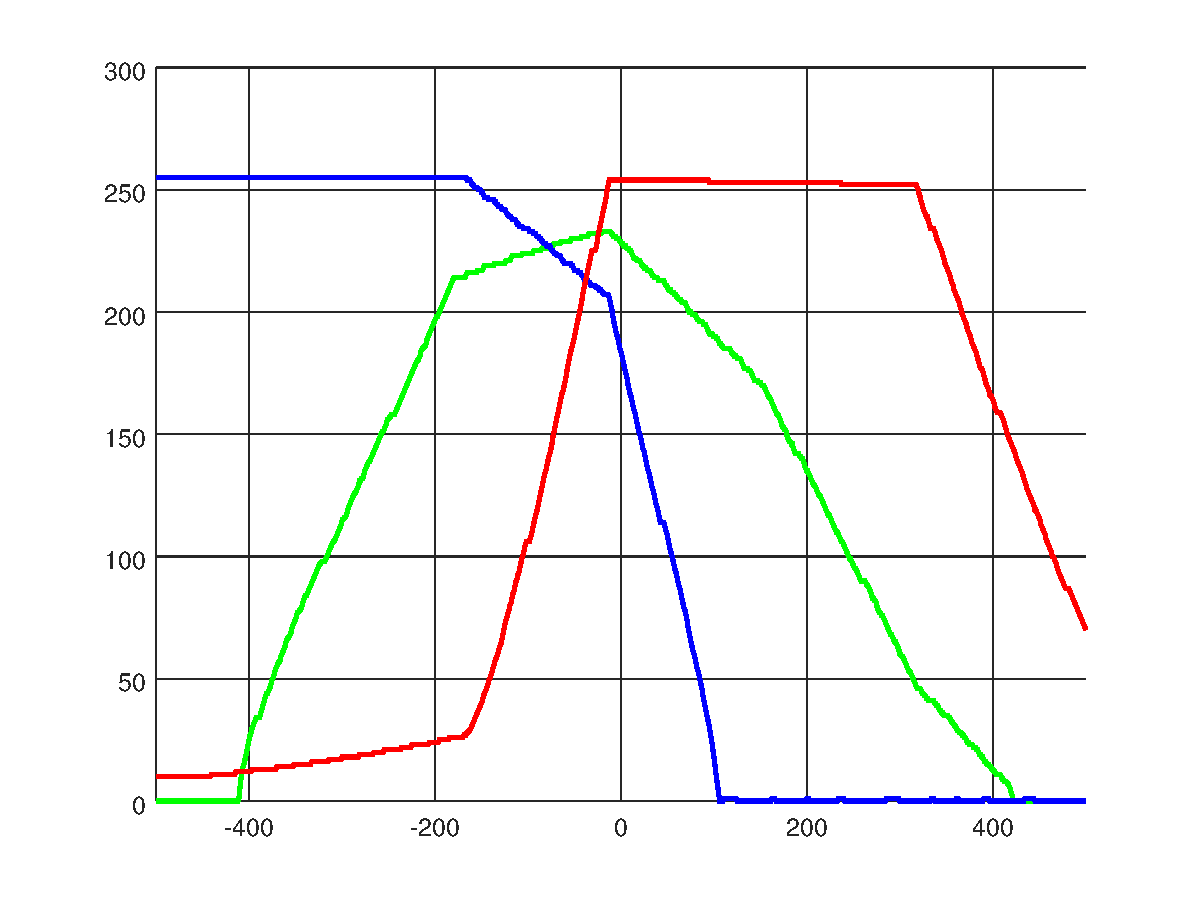
\includegraphics[width=\linewidth]{cmb/converter/rgb-graph.pdf}
		\caption{RGB Profil der Abbildung~\ref{fig:color-strip-orig}.}
		\label{fig:color-strip-orig-rgb}
	\end{subfigure}
\end{figure}

\begin{figure}
	\centering
	\begin{subfigure}
		\centering
		
\includegraphics[width=0.9\linewidth]{cmb/converter/converter-function-strip.png}
		\caption{Der für die Analyse verwendete Farbverlauf.}
		\label{fig:color-strip}
	\end{subfigure}
	\hfill
	\begin{subfigure}
		\centering
		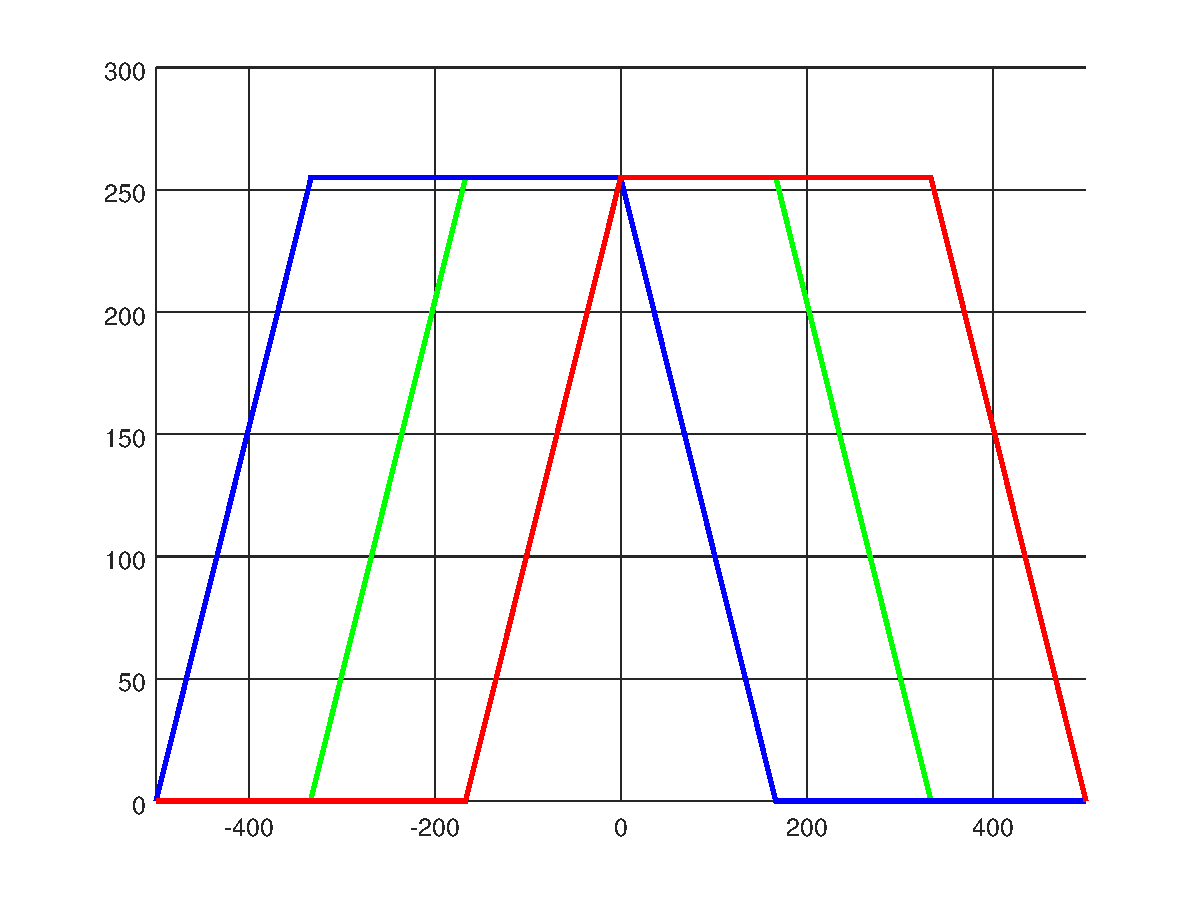
\includegraphics[width=\linewidth]{cmb/converter/converter-function.pdf}
		\caption{RGB Profil der Abbildung~\ref{fig:color-strip}.}
		\label{fig:color-strip-rgb}
	\end{subfigure}
\end{figure}

% TODO: Image CMB (rectangular)
% TODO: Aufzeugung funktion der conversiation RBG -> "Kelvin"